
%% bare_conf.tex
%% V1.4b
%% 2015/08/26
%% by Michael Shell
%% See:
%% http://www.michaelshell.org/
%% for current contact information.
%%
%% This is a skeleton file demonstrating the use of IEEEtran.cls
%% (requires IEEEtran.cls version 1.8b or later) with an IEEE
%% conference paper.
%%
%% Support sites:
%% http://www.michaelshell.org/tex/ieeetran/
%% http://www.ctan.org/pkg/ieeetran
%% and
%% http://www.ieee.org/

\documentclass[conference]{IEEEtran}

% Imports
\usepackage{amsmath}
\usepackage{amsfonts}
\usepackage{amsthm}
% Local
\usepackage{local_macros/isasmathmacros}

% Environments
\theoremstyle{definition}
\newtheorem{definition}{Definition}[section]
\newtheorem{theorem}{Theorem}[section]

\theoremstyle{remark}
\newtheorem*{remark}{Remark}

% correct bad hyphenation here
\hyphenation{op-tical net-works semi-conduc-tor}


\begin{document}

% paper title
\title{Privileged Estimate Fusion With Correlated Gaussian Keystreams}

\author{\IEEEauthorblockN{Marko Ristic}
\IEEEauthorblockA{Autonomous Multisensor Systems Group (AMS),\\
Institute for Intelligent Cooperating Systems (ICS),\\
Otto von Guericke University (OVGU),\\
Magdeburg, Germany\\
Email: marko.ristic@ovgu.de}
\and
\IEEEauthorblockN{Benjamin Noack}
\IEEEauthorblockA{Autonomous Multisensor Systems Group (AMS),\\
Institute for Intelligent Cooperating Systems (ICS),\\
Otto von Guericke University (OVGU),\\
Magdeburg, Germany\\
Email: benjamin.noack@ovgu.de}}

% make the title area
\maketitle

% 
%        d8888 888888b.    .d8888b.  
%       d88888 888  "88b  d88P  Y88b 
%      d88P888 888  .88P  Y88b.      
%     d88P 888 8888888K.   "Y888b.   
%    d88P  888 888  "Y88b     "Y88b. 
%   d88P   888 888    888       "888 
%  d8888888888 888   d88P Y88b  d88P 
% d88P     888 8888888P"   "Y8888P"  
%                                    
%                                    
%                                    
% 

% As a general rule, do not put math, special symbols or citations in the abstract
\begin{abstract}
Providing cryptographic privacy guarantees in a distributed state estimation problem has been a growing topic of research since the ubiquity of modern public networks. One such guarantee is having different levels of estimation performance achievable by trusted and untrusted users within a sensor network. In the presence of multiple sensor measurements, guaranteeing better estimation performance by the usual means of adding removable noise to measurements is complicated by an alternative for untrusted users to improve their performance: fusing more measurements. Our novel method adds correlated noise at different sensors, restricting the performance gained from fusing additional measurements while guaranteeing better performance to those that can remove it. We extend a cryptographic framework for defining estimation privilege and use this to prove the scheme's security goals, while simulations demonstrate the effects of parameters in a concrete estimation problem. A scheme that can ensure such differences in estimation performance between types of estimators can find applications in priority-based or subscription-based performances in environments where more than one sensor is present.
\end{abstract}

% no keywords

\IEEEpeerreviewmaketitle

% 
% 8888888 888b    888 88888888888 8888888b.   .d88888b.  
%   888   8888b   888     888     888   Y88b d88P" "Y88b 
%   888   88888b  888     888     888    888 888     888 
%   888   888Y88b 888     888     888   d88P 888     888 
%   888   888 Y88b888     888     8888888P"  888     888 
%   888   888  Y88888     888     888 T88b   888     888 
%   888   888   Y8888     888     888  T88b  Y88b. .d88P 
% 8888888 888    Y888     888     888   T88b  "Y88888P"  
%                                                        
%                                                        
%                                                        
% 

\section{Introduction}\label{sec:intro}
Sensor data processing and state estimation have long been active areas of research and continue to find applications in modern systems \cite{andersonOptimalFiltering1979,simonOptimalStateEstimation2006}. In the context of distributed sensing environments such as decentralised autonomous vehicles or distributed weather stations, estimation methods relying on Kalman filters and derivatives \cite{haugBayesianEstimationTracking2012} are particular prevalent due to their recursive, often optimal, estimation properties and their suitability to modelling measurement cross-correlations typically required for data fusion \cite{mutambaraDecentralizedEstimationControl1998,ligginsDistributedDataFusion2012}. In recent years, the ubiquity of distributed public networks has seen the additional requirements of preserving algorithm participants' privacies, such as individual contributions or identifying information, become increasingly relevant and has led to an active field of research \cite{renSecurityChallengesPublic2012,brennerSecretProgramExecution2011}.

While hiding only transmitted information from eavesdroppers can be achieved using common private or public key encryption schemes \cite{katzIntroductionModernCryptography2008}, distributed estimation tasks that preserve participants' privacies require information to remain hidden during partial or complete processing of the task and often justify some leakage \cite{risticSecureFastCovariance2021,shiPrivacyPreservingAggregationTimeSeries2011}. The security goals of these problems are context-specific and have produced a variety of solutions. In \cite{alanwarPrOLocResilientLocalization2017}, non-Bayesian localisation is performed using homomorphic encryption such that individual sensor information and measurements remain private, while in \cite{aristovEncryptedMultisensorInformation2018}, similar goals are achieved in a Bayesian setting by fusing linear measurements when sensors form a hierarchical network. A combination of homomorphic and order-revealing encryption schemes are used in \cite{risticSecureFastCovariance2021} to solve conservative Gaussian estimate fusion while leaking only the ratios of estimate covariances, and in \cite{shiPrivacyPreservingAggregationTimeSeries2011,joyeScalableSchemePrivacyPreserving2013}, cryptographic aggregation schemes are introduced and used to leak only total consumptions in an energy grid while hiding individual participant power-usages. In addition to these examples of privacy, optimal estimation performance can itself also be considered leakage, introducing an idea of privilege in estimation, where leakage captures the difference in performance between trusted and untrusted estimators. In the original Global Positioning System (GPS) \cite{grovesPrinciplesGNSSInertial2015}, this was achieved with a secondary encrypted channel that allowed better estimation performance to parties that held an encryption key. Similarly, in \cite{murguiaInformationTheoreticPrivacyChaos2020}, a synchronised chaotic system is used to add noise to measurements which can only be removed by estimators knowing its properties. This idea of estimation privilege is further explored in \cite{risticCryptographicallyPrivilegedState2022}, where a relevant formal cryptographic definition is given and a scheme for a single sensor presented. Here, a synchronised pseudorandom Gaussian keystream adds measurement noise only removable by estimators holding the stream key.

In this work, we consider the definition of estimation privilege presented in \cite{risticCryptographicallyPrivilegedState2022} and introduce a modified scheme suitable for an environment of multiple sensors, where both holding the secret key and fusing additional measurements can lead to better estimation performance. Our contribution consists of a generalised notion of estimation privilege, the introduction of security requirements for privileged estimation in a well defined multisensor environment and a scheme that satisfies them. Along with a cryptographic proof sketch, simulation results are provided to demonstrate the effects of scheme parameters and how they can be chosen to provide varying amounts of privilege. Use-cases for varying performance in this way include subscription or priority models where some users are provided better results than others. For example, subscription-based weather forecasts using measurements from spatially distributed stations or modular mass-produced sensors that differ in accuracy dependent on cost.

In section \ref{sec:prob}, the multisensor estimation privilege problem is presented. Relevant preliminaries are introduced in section \ref{sec:prelim} and the estimation privilege fusion scheme itself in section \ref{sec:scheme}. A cryptographic analysis and the simulation results are then given in sections \ref{sec:crypto} and \ref{sec:sim}, respectively, before the concluding remarks in section \ref{sec:conc}.

% 
% ##    ##  #######  ########    ###    ######## ####  #######  ##    ## 
% ###   ## ##     ##    ##      ## ##      ##     ##  ##     ## ###   ## 
% ####  ## ##     ##    ##     ##   ##     ##     ##  ##     ## ####  ## 
% ## ## ## ##     ##    ##    ##     ##    ##     ##  ##     ## ## ## ## 
% ##  #### ##     ##    ##    #########    ##     ##  ##     ## ##  #### 
% ##   ### ##     ##    ##    ##     ##    ##     ##  ##     ## ##   ### 
% ##    ##  #######     ##    ##     ##    ##    ####  #######  ##    ## 
% 

\subsection{Notation}\label{subsec:notation}
Lowercase underlined characters $\vec{v}$ are vectors and uppercase bold characters $\mat{M}$ are matrices, while $\vec{0}$, $\mat{0}$ and $\mat{I}$ are the zero vector, zero matrix and identity matrix, respectively, with sizes inferrable from context. $\mat{M}\succ 0$ and $\mat{M}\succeq 0$ denote positive definitness and semi-definitness, respectively, and $\mat{M}\succ \mat{N}$ is short for $\mat{M} - \mat{N} \succ 0$. Given an indexed vector $\vec{v}_i$, notation $\vec{v}^{(a:b)}$, $a<b$, will denote the stacked vector $[\vec{v}_a\ \vec{v}_{a+1}\ \cdots\ \vec{v}_b]^\top$, while for indexed matrices $\mat{M}_i$, $\mat{M}^{(a:b)}$ will denote the block-diagonal matrix with the indexed matrices along the diagonal. Function $\mathsf{Cov}[\cdot]$ computes the covariance of a random vector, $\sim$ denotes distribution, $\dot{\sim}$ denotes pseudorandom distribution and, in a cryptographic context, $\mathcal{A}(\vec{v})$ denotes the output of an arbitrary algorithm $\mathcal{A}$ given inputs $\vec{v}$.

% 
% 8888888b.  8888888b.   .d88888b.  888888b.   
% 888   Y88b 888   Y88b d88P" "Y88b 888  "88b  
% 888    888 888    888 888     888 888  .88P  
% 888   d88P 888   d88P 888     888 8888888K.  
% 8888888P"  8888888P"  888     888 888  "Y88b 
% 888        888 T88b   888     888 888    888 
% 888        888  T88b  Y88b. .d88P 888   d88P 
% 888        888   T88b  "Y88888P"  8888888P"  
%                                              
%                                              
%                                              
% 

\section{Problem Formulation}\label{sec:prob}
We are interested in environments where multiple sensors are present and the fusion of their measurements can lead to better state estimation accuracy of the system they are measuring. In these environments, we want to provide levels of privilege to state estimators such those with a higher privilege can perform better than those with a lower one, while taking into consideration the estimation benefits from fusing additional measurements. We will consider linear and Gaussian models, where a state $\vec{x}_k \in \mathbb{R}^n$, at an integer timestep $k$, follows a system model given by
\begin{equation}\label{eqn:system_model}
  \vec{x}_k = \mat{F}_k \vec{x}_{k-1} + \vec{w}_k\,,
\end{equation}
with white noise term $\vec{w}_k \sim \mathcal{N}(\vec{0},\mat{Q}_k)$ and a known covariance $\mat{Q}_k \in \mathbb{R}^{n \times n}$. Similarly, measurements $\vec{y}_{k,i} \in \mathbb{R}^m$ from each sensor $i$, $1\leq i\leq N$, follow the measurement models
\begin{equation}\label{eqn:measurement_models}
  \vec{y}_{k,i} = \mat{H}_{k,i} \vec{x}_k + \vec{v}_{k,i}\,,
\end{equation}
with white noise term $\vec{v}_{k,i} \sim \mathcal{N}(\vec{0},\mat{R}_{k,i})$ and a known covariance $\mat{R}_{k,i} \in \mathbb{R}^{m \times m}$. In addition to these models, we assume that all sensors $i$ are synchronised in timesteps $k$ to simplify later cryptographic evaluation. In practice, this would restrict the presented schemes to scenarios where synchronisation is easier to guarantee, such as ones where measurements are taken infrequently.

Each of the sensors also holds a secret key $\mathsf{sk}_i$, which can be made available to estimators of appropriate privilege. The privileges that we consider, in terms of access to keys and measurements, will be defined by sequential sensors. That is, in the presence of $N$ sensors, we consider exactly $N$ possible privilege levels, where each privilege $p>0$ corresponds to holding the sequential secret keys $\mathsf{sk}_j$, $1\leq j \leq p$, while being unprivileged, $p=0$, corresponds to holding none. We assume that estimators have access to all ``privileged measurements'', those from sensors whose keys they hold, and can additionally fuse ``unprivileged measurements'' from those whose keys they do not hold. To simplify notation, we will consider access to unprivileged measurements to be sequential as well, and can therefore capture their capabilities by letting $\mathsf{e}^{[p,q]}$ denote an estimator with privilege $p$ and access to measurements from $q\geq p$ sensors $i$, $1\leq i \leq q$.

To cryptographically guarantee the difference between estimation performances, we will use the notion of covariance privilege \cite{risticCryptographicallyPrivilegedState2022}. As we desire better performance for higher privilege estimators as well as to limit the gained performance from fusing unprivileged measurements, two differences will be considered.
\begin{LaTeXdescription}
  \item[Different Keys Lower Bound] We want to guarantee a lower bound on the estimation degradation of any unprivileged estimator $\mathsf{e}^{[0,N]}$ on all privilege-$p$ estimators $\mathsf{e}^{[p,p]}$. Naturaly, this will remain a lower bound when unprivileged estimators have access to fewer unprivileged measurements or privileged estimators have access to more.
  \item[Same Keys Upper Bound] We want to guarantee an upper bound on the estimation gain any estimator $\mathsf{e}^{[p,N]}$ has on all privilege-$p$ estimators $\mathsf{e}^{[p,p]}$. Here, the bound will remain an upper bound when fewer unprivileged measurements are fused.
\end{LaTeXdescription}
The resulting scheme should be such that two parameters are responsible for choosing the values of these two bounds.
\begin{remark}
  We stress that the two bounds that will be guaranteed only bound the performances of estimators of the specified forms. That is, nothing is said about estimators which may corrupt sensors to obtain keys beyond their privilege or additional unprivileged measurements. Bounds on leakage caused by corrupting sensors can in some cases by captured by estimators of a new form $\mathsf{e}^{[p^\prime,q^\prime]}$, but are in general beyond the scope of this work.
\end{remark}

% 
% 8888888b.  8888888b.  8888888888 888      8888888 888b     d888 
% 888   Y88b 888   Y88b 888        888        888   8888b   d8888 
% 888    888 888    888 888        888        888   88888b.d88888 
% 888   d88P 888   d88P 8888888    888        888   888Y88888P888 
% 8888888P"  8888888P"  888        888        888   888 Y888P 888 
% 888        888 T88b   888        888        888   888  Y8P  888 
% 888        888  T88b  888        888        888   888   "   888 
% 888        888   T88b 8888888888 88888888 8888888 888       888 
%                                                                 
%                                                                 
%                                                                 
% 

\section{Preliminaries}\label{sec:prelim}
When defining our scheme and discussing its cryptographic guarantees, we will make use of Gaussian keystreams and the notion of cryptographic estimation covariance privilege. These have been summarised below.

% 
% ##    ## ######## ##    ##  ######  ######## ########  ########    ###    ##     ## 
% ##   ##  ##        ##  ##  ##    ##    ##    ##     ## ##         ## ##   ###   ### 
% ##  ##   ##         ####   ##          ##    ##     ## ##        ##   ##  #### #### 
% #####    ######      ##     ######     ##    ########  ######   ##     ## ## ### ## 
% ##  ##   ##          ##          ##    ##    ##   ##   ##       ######### ##     ## 
% ##   ##  ##          ##    ##    ##    ##    ##    ##  ##       ##     ## ##     ## 
% ##    ## ########    ##     ######     ##    ##     ## ######## ##     ## ##     ## 
% 

\subsection{Gaussian keystreams}\label{subsec:gauss_keystreams}
A Gaussian keystream is a sequence of pseudorandom multivariate Gaussian samples $\vec{g}_k\in\mathbb{R}^m\ \dot{\sim}\ \mathcal{N}(\vec{0},\mat{S})$, $k>0$, generated using a secret key, for some covariance matrix $\mat{S}$. The sequence is indistinguishable from a truly random multivariate Gaussian sequence to any observer who does not hold the key while being reproducible exactly by those that do. The keystream can be constructed from a typical cryptographic stream cipher \cite[Ch. 3.6]{katzIntroductionModernCryptography2008}, by first using any common method for random floating-point generation \cite{goualardGeneratingRandomFloatingPoint2020} to create a stream of pseudorandom uniform samples $u_x\ \dot{\sim}\ \mathcal{U}(0,1)$, $x>0$. Here, we make the assumption that floating-point representations of real numbers are sufficiently similar to actual real numbers, made reasonable in practice due to the insignificance of their difference in many applications and their prevalence in estimation theory.

To construct the Gaussian keystream $\vec{g}_k$, $k>0$, from the uniform one $u_x$, $x>0$, a vector of uncorrelated standard Gaussian samples $\vec{z}_k$ is first generated using the Box-Muller transform,
\begin{equation}\label{eqn:standard_gaussian_generation}
    \vec{z}_k = 
  \begin{bmatrix}
    z_{(k-1)m+1} & \cdots & z_{km}
  \end{bmatrix}^\top
\end{equation}
where 
\begin{equation*}
  z_x =
  \begin{cases}
    \sqrt{-2\ln(u_{2x})}\cos(2\pi u_{2x+1}), & x \text{ is odd}\\
    \sqrt{-2\ln(u_{2x})}\sin(2\pi u_{2x+1}), & x \text{ is even}\\
  \end{cases}\,,
\end{equation*}
and then correlated by
\begin{equation}\label{eqn:gaussian_keystream_generation}
    \vec{g}_k = \mat{S}^\frac{1}{2}\vec{z}_k\,,
\end{equation}
where $\mat{S}^\frac{1}{2}$ is any matrix such that $\mat{S}^\frac{1}{2}\mat{S}^{\frac{1}{2}\top} = \mat{S}$.

% 
% ########  ########  #### ##     ##    ########  ######## ######## 
% ##     ## ##     ##  ##  ##     ##    ##     ## ##       ##       
% ##     ## ##     ##  ##  ##     ##    ##     ## ##       ##       
% ########  ########   ##  ##     ##    ##     ## ######   ######   
% ##        ##   ##    ##   ##   ##     ##     ## ##       ##       
% ##        ##    ##   ##    ## ##      ##     ## ##       ##       
% ##        ##     ## ####    ###       ########  ######## ##       
% 

\subsection{Cryptographic Estimation Privilege}\label{subsec:crypto_privilege}
The formal definition of a privileged estimation scheme and accompanying notion of covariance privilege are introduced in \cite{risticCryptographicallyPrivilegedState2022} and capture a reduction in estimation performance that can always be achieved from a probabilistic polynomial-time (PPT) estimator knowing only unprivileged measurements, and holding no scheme key, to one knowing both the key and privileged measurements. We will use a slight generalisation of this definition to capture an arbitrary difference that can always be achieved between the estimators (rather than only a reduction).
A privileged estimation scheme is defined by a pair of probabilistic algorithms $(\mathsf{Setup}, \mathsf{Noise})$:
\begin{LaTeXdescription}
  \item[$\mathsf{Setup}(\mathcal{M}_S,\mathcal{M}_M,\kappa)$] Given system and measurement models $\mathcal{M}_S$ and $\mathcal{M}_M$, and the security parameter $\kappa$, public parameters $\mathsf{pub}$ and a secrect key $\mathsf{sk}$ are returned.
  \item[$\mathsf{Noise}(\mathsf{pub},\mathsf{sk},k,\mathcal{M}_S,\mathcal{M}_M,\vec{y}_1,\dots,\vec{y}_k)$] Given public parameters $\mathsf{pub}$, secret key $\mathsf{sk}$, timestep $k$, models $\mathcal{M}_S$ and $\mathcal{M}_M$, and measurements $\vec{y}_1,\dots,\vec{y}_k$, modified privileged and unprivileged measurements, $\vec{y}^{[\mathsf{p}]}_k$ and $\vec{y}^{[\mathsf{up}]}_k$, respectively, are returned.
\end{LaTeXdescription}
Using the defintions from \cite{risticCryptographicallyPrivilegedState2022} for an \textit{estimator} and \textit{negligible covariance} $\mathsf{neglCov}_m(\kappa)$, the notion of covariance privilege is defined as follows.
\begin{definition}\label{def:cov_priv_security_notion}
  A privileged estimation scheme meets notion \textit{$\{\mat{D}_1,\mat{D}_2,\dots\}$-Covariance Privilege for Models $\mathcal{M}_S$ and $\mathcal{M}_M$} if for any PPT estimator $\mathcal{A}$, there exists a PPT estimator $\mathcal{A}^\prime$, such that
  \begin{equation}
    \begin{split}
      &\mathsf{Cov}\left[\mathcal{A}\left(k,\kappa,\mathsf{pub},\mathcal{M}_S,\mathcal{M}_M,\vec{y}^{[\mathsf{up}]}_1,\dots,\vec{y}^{[\mathsf{up}]}_k\right) - \vec{x}_k\right]\\
      &-\mathsf{Cov}\left[\mathcal{A}^\prime\left(k,\kappa,\mathsf{pub},\mathcal{M}_S,\mathcal{M}_M,\vec{y}^{[\mathsf{p}]}_1,\dots,\vec{y}^{[\mathsf{p}]}_k\right) - \vec{x}_k\right]\\
      &\quad\succeq \mat{D}_k - \mathsf{neglCov}_m(\kappa)
    \end{split}
  \end{equation}
  for all $k>0$, some negligible covariance and where matrices $\mat{D}_k$ are semi-definite, \textit{i.e.}, $\mat{D}_k \preceq \mat{0}$ or $\mat{D}_k \succeq \mat{0}$. Here, $\mathcal{A}$ and $\mathcal{A}^\prime$ are running in polynomial-time with respect to the parameter $\kappa$ and all probabilities are taken over randomness introduced in models $\mathcal{M}_S$ and $\mathcal{M}_M$, estimators $\mathcal{A}$ and $\mathcal{A}^\prime$, and algorithms $\mathsf{Setup}$ and $\mathsf{Noise}$.
\end{definition}

We note that in the generalised notion, definition \ref{def:cov_priv_security_notion}, $\mat{D}_k\preceq \mat{0}$ is allowed, and unprivileged estimators may perform better than privileged ones, albeit by a bounded amount. This feature will be useful when discussing additional estimation performance gainable from fusing unprivileged measurements. Lastly, a sign is also corrected, such that negligible covariances are subtracted (rather than added), correctly capturing the additional negligible performance gainable by an unprivileged estimator.

% 
%  .d8888b.   .d8888b.  888    888 8888888888 888b     d888 8888888888 
% d88P  Y88b d88P  Y88b 888    888 888        8888b   d8888 888        
% Y88b.      888    888 888    888 888        88888b.d88888 888        
%  "Y888b.   888        8888888888 8888888    888Y88888P888 8888888    
%     "Y88b. 888        888    888 888        888 Y888P 888 888        
%       "888 888    888 888    888 888        888  Y8P  888 888        
% Y88b  d88P Y88b  d88P 888    888 888        888   "   888 888        
%  "Y8888P"   "Y8888P"  888    888 8888888888 888       888 8888888888 
%                                                                      
%                                                                      
%                                                                      
% 

\section{Privileged Fusion}\label{sec:scheme}
The idea behind our privileged estimation fusion scheme is to add \textit{correlated} Gaussian keystreams to the measurements from each sensor. These noises can be computed and subtracted by estimators holding respective sensor keys, while their correlation limits the additional information gained from fusing unprivileged measurements. 

% 
% ##    ##  #######  ####  ######  ########     ######   ######## ##    ## 
% ###   ## ##     ##  ##  ##    ## ##          ##    ##  ##       ###   ## 
% ####  ## ##     ##  ##  ##       ##          ##        ##       ####  ## 
% ## ## ## ##     ##  ##   ######  ######      ##   #### ######   ## ## ## 
% ##  #### ##     ##  ##        ## ##          ##    ##  ##       ##  #### 
% ##   ### ##     ##  ##  ##    ## ##          ##    ##  ##       ##   ### 
% ##    ##  #######  ####  ######  ########     ######   ######## ##    ## 
% 

\subsection{Noise Generation}\label{subsec:noise_gen}
Similarly to the Gaussian keystream generation in \eqref{eqn:gaussian_keystream_generation}, pseudorandom samples can be correlated in this way even when generated using different stream cipher keys. To parameterise the correlation between noises at each sensor, we introduce a fully correlated component $\mat{Z}\in\mathbb{R}^{m\times m}$ and an uncorrelated component $\mat{Y}\in\mathbb{R}^{m\times m}$ and define a noise cross-correlation matrix for $x$ noises as $\mat{S}^{(x)} \in \mathbb{R}^{xm\times xm}$,
\begin{equation}\label{eqn:noise_correlation_matrix}
  \mat{S}^{(x)}=
  \begin{bmatrix}
    \mat{Z} & \cdots & \mat{Z}\\
    \vdots & \ddots & \vdots\\
    \mat{Z} & \cdots & \mat{Z}\\
  \end{bmatrix}+
  \begin{bmatrix}
    \mat{Y} & \mat{0} & \mat{0}\\
    \mat{0} & \ddots & \mat{0}\\
    \mat{0} & \mat{0} & \mat{Y}\\
  \end{bmatrix}\,,
\end{equation}
and $\mat{S}^{(1)}=\mat{Z}+\mat{Y}$. The generation of all $N$ multivariate Gaussian noises at timestep $k$, $\vec{g}_k^{(1:N)}$, can now be written as
\begin{equation}\label{eqn:all_correlated_noises_generation}
  \vec{g}_k^{(1:N)}=
  \begin{bmatrix}
    \vec{g}_{k,1}\\
    \vdots\\
    \vec{g}_{k,N}
  \end{bmatrix}=
  \mat{S}^{(N)\frac{1}{2}}\cdot
  \begin{bmatrix}
    \vec{z}_{k,1}\\
    \vdots\\
    \vec{z}_{k,N}
  \end{bmatrix}\,,
\end{equation}
where each $\vec{z}_{k,i}$ is computed as $\vec{z}_k$ in \eqref{eqn:standard_gaussian_generation} using uniform samples generated with key $\mathsf{sk}_i$, and $\mat{S}^{(N)\frac{1}{2}}$ is a matrix such that $\mat{S}^{(N)\frac{1}{2}}\mat{S}^{(N)\frac{1}{2}\top}=\mat{S}^{(N)}$. Notably, it is important that the first $p$ noises $\vec{g}_{k,i}$, $1\leq i \leq p$, in \eqref{eqn:all_correlated_noises_generation}, denoted $\vec{g}_k^{(1:p)}$, can be reproduced by an estimator of privilege $p$, holding only the keys $\mathsf{sk}_i$, $1\leq i \leq p$. One case where this is possible is when a lower-triangular decomposition, such as the the Cholesky decomposition, is used to compute $\mat{S}^{(x)\frac{1}{2}}$ from $\mat{S}^{(x)}$. Here, each correlated Gaussian sample $\vec{g}_{k,i}$ is computable from preceeding uniform samples $\vec{z}_{k,j}$, $j\leq i$ only, and the generalised noise generation equation
\begin{equation}\label{eqn:p_correlated_noises_generation}
  \vec{g}_k^{(1:p)}=
  \mat{S}^{(p)\frac{1}{2}}\cdot
  \begin{bmatrix}
    \vec{z}_{k,1}\\
    \vdots\\
    \vec{z}_{k,p}
  \end{bmatrix}\,,
\end{equation}
generates the same first $p$ noises $\vec{g}_k^{(1:p)}$ as would be obtained from \eqref{eqn:all_correlated_noises_generation} since $\mat{S}^{(p)\frac{1}{2}}\in\mathbb{R}^{pm\times pm}$ is equal to the top left block of matrix $\mat{S}^{(N)\frac{1}{2}}$ when using the Cholesky decomposition.

With \eqref{eqn:p_correlated_noises_generation}, at every timestep $k$, $\vec{g}_k^{(1:N)}$ can be generated using all $N$ keys and used to modify sensor measurements, while the subset $\vec{g}_k^{(1:p)}$ can be generated by estimators of privilege $p$ using only the keys they hold.

% 
% ##     ##  #######  ########  ######## ##          ##     ##  #######  ########  
% ###   ### ##     ## ##     ## ##       ##          ###   ### ##     ## ##     ## 
% #### #### ##     ## ##     ## ##       ##          #### #### ##     ## ##     ## 
% ## ### ## ##     ## ##     ## ######   ##          ## ### ## ##     ## ##     ## 
% ##     ## ##     ## ##     ## ##       ##          ##     ## ##     ## ##     ## 
% ##     ## ##     ## ##     ## ##       ##          ##     ## ##     ## ##     ## 
% ##     ##  #######  ########  ######## ########    ##     ##  #######  ########  
% 

\subsection{Measurement Modification}
With a way to generate noises for sensors and estimators, we can introduce the means of measurement modification and the observable measurement models for different estimators. Measurement modification is peformed by adding noises $\vec{g}_k^{(1:N)}$ to measurements from each sensor $i$ before making them public, resulting in modified measurement equations for each sensor,
\begin{equation}\label{eqn:modified_measurement}
\begin{split}
  \vec{y}_{k,i}^\prime &= \vec{y}_{k,i} + \vec{g}_{k,i}\\
  &= \mat{H}_{k,i}\vec{x}_k + \vec{v}_{k,i} + \vec{g}_{k,i}\,,
\end{split}
\end{equation}
with real measurement noise $\vec{v}_{k,i}\sim\mathcal{N}(\vec{0},\mat{R}_{k,i})$ and the vector of all added noises $\vec{g}_k^{(1:N)}\ \dot{\sim}\ \mathcal{N}(\vec{0}, \mat{S}^{(N)})$. As we assume that sensors are synchronised, we can capture the correlation between these modified measurements exactly by considering the stacked measurement model for any estimator with access to $q$ measurements, $\mathsf{e}^{[p,q]}$, at time $k$, given by
\begin{equation}\label{eqn:measurement_equation}
  \begin{split}
    \vec{y}_k^{\prime(1:q)} &= \vec{y}_k^{(1:q)} + \vec{g}_k^{(1:q)}\\
    &= \mat{H}_k^{(1:q)}\vec{x}_k + \vec{v}_k^{(1:q)} + \vec{g}_k^{(1:q)}
  \end{split}
\end{equation}
where $\vec{v}_k^{(1:q)}\sim\mathcal{N}(\vec{0},\mat{R}_k^{(1:q)})$ and $\vec{g}_k^{(1:q)}\ \dot{\sim}\ \mathcal{N}(\vec{0},\mat{S}^{(q)})$, with
\begin{equation*}
  \vec{y}_k^{\prime(1:q)}=
  \begin{bmatrix}
    \vec{y}_{k,1}^\prime\\
    \vdots\\
    \vec{y}_{k,q}^\prime
  \end{bmatrix},\ 
  \vec{y}_k^{(1:q)}=
  \begin{bmatrix}
    \vec{y}_{k,1}\\
    \vdots\\
    \vec{y}_{k,q}
  \end{bmatrix},\ 
  \mat{H}_k^{(1:q)}=
  \begin{bmatrix}
    \mat{H}_{k,1}\\
    \vdots\\
    \mat{H}_{k,q}\\
  \end{bmatrix}\,,
\end{equation*}
\begin{equation*}
  \vec{v}_k^{(1:q)}=
  \begin{bmatrix}
    \vec{v}_{k,1}\\
    \vdots\\
    \vec{v}_{k,q}
  \end{bmatrix},\ 
  \mat{R}_k^{(1:q)}=
    \begin{bmatrix}
      \mat{R}_{k,1} & \mat{0} & \mat{0}\\
      \mat{0} & \ddots & \mat{0}\\
      \mat{0} & \mat{0} & \mat{R}_{k,q}
    \end{bmatrix}\,
\end{equation*}
and $\mat{S}^{(q)} \in \mathbb{R}^{qm\times qm}$ defined by \eqref{eqn:noise_correlation_matrix}.

Since we are using a cryptographically sound stream cipher to generate the added Gaussian keystream, the pseudorandom samples are indistinguishable from truly random ones to estimators without appropriate keys, which leads us to three observable measurement models, \textit{i.e.}, the models that capture all the information available to an estimator exactly, for three types of mutually exhaustive estimators.
\begin{LaTeXdescription}
  \item[Estimators of the form $\mathsf{e}^{[0,q]}$] Here, no keys are held by the unprivileged estimators and the generated noise $\vec{g}_k^{(1:q)}$ is indistinguishable from noise from the truly random distribution $\mathcal{N}(\vec{0}, \mat{S}^{(q)})$. For these estimators, we can rewrite the measurement equation \eqref{eqn:measurement_equation} as the observed measurement model
  \begin{equation}\label{eqn:0q_obs_measurement_model}
    \vec{y}_k^{[0,q]} = \mat{H}_k^{(1:q)}\vec{x}_k + \vec{v}_k^{\prime}\,,
  \end{equation}
  with truly Gaussian term $\vec{v}_k^{\prime} \sim \mathcal{N}(\vec{0}, \mat{R}_k^{(1:q)}+\mat{S}^{(q)})$.
  
  \item[Estimators of the form $\mathsf{e}^{[p,p]}$] Estimators with keys for all the sensors to which they have access can generate all added noises and subtract them from the recieved measurements. That is, $\vec{g}_k^{(1:p)}$ can be generated and $\vec{y}_k^{[p,p]}=\vec{y}_k^{\prime(1:p)}-\vec{g}_k^{(1:p)}$ computed to give the observed measurement model equal to recieving unmodified measurements only,
  \begin{equation}\label{eqn:pp_obs_measurement_model}
    \vec{y}_k^{[p,p]} = \mat{H}_k^{(1:p)}\vec{x}_k + \vec{v}_k^{(1:p)}\,,
  \end{equation}
  where $\vec{v}_k^{(1:p)} \sim \mathcal{N}(\vec{0}, \mat{R}_k^{(1:p)})$.

  \item[Estimators of the form $\mathsf{e}^{[p,q]}$, $p<q$] Lastly, we want the observed measurement model when only some accessible measurements can have have their noises removed. Here, care must be taken when giving the observed model, as the noises from sensors $i>p$, which cannot be removed, are conditionally dependant on the known noises $\vec{g}_k^{(1:p)}$. Since we can generate the noises $\vec{g}_k^{(1:p)}$ and know that $\vec{g}_k^{(1:q)}\ \dot{\sim}\ \mathcal{N}(\vec{0}, \mat{S}^{(q)})$, we can write 
  \begin{equation}\label{eqn:block_noises_and_correlation}
    \begin{split}
      &\vec{g}_k^{(1:q)}=
      \begin{bmatrix}
        \vec{g}_k^{(1:p)}\\
        \vec{g}_k^{(p+1:q)}\\
      \end{bmatrix}\\ 
      &\qquad \dot{\sim}\ \mathcal{N}\left(
      \begin{bmatrix}
        \vec{0}\\
        \vec{0}
      \end{bmatrix},\mat{S}^{(q)}=
      \begin{bmatrix}
        \mat{S}^{(p)} & \mat{Z}^\prime\\
        \mat{Z}^{\prime\top} & \mat{S}^{(q-p)}
      \end{bmatrix}\right)\,,
    \end{split}
  \end{equation}
  where $\mat{Z}^\prime \in \mathbb{R}^{pm \times (q-p)m}$ is a block matrix with every block equal to $\mat{Z}$, and compute the conditional pseudorandom Gaussian distribution
  \begin{equation}\label{eqn:conditional_noise_distribution}
    \begin{split}
      &\vec{g}_k^{(p+1:q)} \mid \vec{g}_k^{(1:p)}\\
      &\qquad \dot{\sim}\ \mathcal{N}\Big(\mat{Z}^{\prime\top}\mat{S}^{(p)-1}\vec{g}_k^{(1:p)},\\
      &\qquad\qquad \mat{S}^{(q-p)} - \mat{Z}^{\prime\top}\mat{S}^{(p)-1}\mat{Z}^{\prime}\Big)\,.
    \end{split}
  \end{equation}
  Now, subtracting the known noises $\vec{g}_k^{(1:p)}$ and the means of unknown noises \eqref{eqn:conditional_noise_distribution} from recieved measurements,
  \begin{equation}\label{eqn:pq_measurement_offset}
    \vec{y}_k^{[p,q]}=\vec{y}_k^{\prime(1:q)} - 
    \begin{bmatrix}
      \vec{g}_k^{(1:p)}\\
      \mat{Z}^{\prime\top}\mat{S}^{(p)-1}\vec{g}_k^{(1:p)}
    \end{bmatrix}\,,
  \end{equation}
  and accounting for unknown pseudorandom noises being indistinguishable from random, a zero-mean observed measurement model can be written as
  \begin{equation}\label{eqn:pq_obs_measurement_model}
    \vec{y}_k^{[p,q]} = \mat{H}_k^{(1:q)}\vec{x}_k + \vec{v}_k^{\prime}
  \end{equation}
  where 
  \begin{equation*}
    \begin{split}
      &\vec{v}_k^{\prime} \sim \mathcal{N}\Bigg(\vec{0},\\
      &\qquad 
      \begin{bmatrix}
        \mat{R}_k^{(1:p)} & \mat{0}\\
        \mat{0} & \mat{S}^{(q-p)} - \mat{Z}^{\prime\top}\mat{S}^{(p)-1}\mat{Z}^{\prime} + \mat{R}_k^{(p+1:q)}
      \end{bmatrix}\Bigg).
    \end{split}
  \end{equation*}
\end{LaTeXdescription}
\begin{remark}
  Recalling that access to unprivileged measurements are sequential to simplify notation, \eqref{eqn:block_noises_and_correlation}, \eqref{eqn:pq_measurement_offset} and \eqref{eqn:pq_obs_measurement_model} can be generalised when having access to arbitrary $q-p$ non-sequential unprivileged measurements $\vec{y}_{k,i}$, $p<i\leq q$, by appropriately replacing elements $\mat{Z}^{\prime\top}$ and $\mat{S}^{(q-p)}$ in \eqref{eqn:block_noises_and_correlation}.
\end{remark}

From the observed measurement models \eqref{eqn:0q_obs_measurement_model}, \eqref{eqn:pp_obs_measurement_model} and \eqref{eqn:pq_obs_measurement_model} we can tell that the parameters $\mat{Z}$ and $\mat{Y}$ (within matrices $\mat{S}^{(x)}$) control the difference in estimation performance between the three types of estimators. More specifically, while both components affect estimation, the fully correlated component $\mat{Z}$ predominantly affects the difference in estimation between estimators of the form $\mathsf{e}^{[0,q]}$ and $\mathsf{e}^{[p,p]}$, while the uncorrelated component $\mat{Y}$ affects the difference between estimators $\mathsf{e}^{[p,p]}$ and $\mathsf{e}^{[p,q]}$. These two differences correspond exactly to the differences we wish to cryptographically guarantee from section \ref{sec:prob}. The effects of choosing $\mat{Z}$ and $\mat{Y}$ will be more formally explored in sections \ref{sec:crypto} and \ref{sec:sim}.

% 
% ##    ##  #######  ####  ######  ########    ########  ####  ######  ######## 
% ###   ## ##     ##  ##  ##    ## ##          ##     ##  ##  ##    ##    ##    
% ####  ## ##     ##  ##  ##       ##          ##     ##  ##  ##          ##    
% ## ## ## ##     ##  ##   ######  ######      ##     ##  ##   ######     ##    
% ##  #### ##     ##  ##        ## ##          ##     ##  ##        ##    ##    
% ##   ### ##     ##  ##  ##    ## ##          ##     ##  ##  ##    ##    ##    
% ##    ##  #######  ####  ######  ########    ########  ####  ######     ##    
% 

\subsection{Noise Distribution}\label{subsec:noise_dist}
While we have described a method for generating noises that modify $N$ measurements resulting in different observed measurement models depending on estimator privilege, we have not discussed where the noise is generated and how it is distributed to the sensors. To handle the inherent correlation of the noises $\vec{g}_{k,i}$, $1\leq i \leq N$, used to modify measurements, they can be either generated centrally before distribution to sensors or sequentially at the sensors themselves, given previously generated values.
\begin{LaTeXdescription}
  \item[Central noise generation] To compute noises centrally, \eqref{eqn:p_correlated_noises_generation} can be computed at a single central processor and each noise $\vec{g}_{k,i}$, $1\leq i \leq N$ sent to respective sensors $i$ before modifying their local measurement by \eqref{eqn:modified_measurement}.
  \item[Sequential noise generation] To compute the same noises sequentially, at each timestep $k$, sensor $1$ can generate its noise independently using its current standard Gaussian sample $\vec{z}_{k,1}$, by $\vec{g}_{k,1} = \mat{S}^{(1)\frac{1}{2}}\vec{z}_{k,1}$. Each following sensor $i>1$ can generate its noise $\vec{g}_{k,i}$ given the preceeding noises $\vec{g}_k^{(1:i-1)}$, following the conditional reasoning in \eqref{eqn:conditional_noise_distribution}, allowing for the generation of $\vec{g}_{k,i}$ with the transformation
  \begin{equation}
    \begin{split}
      \vec{g}_{k,i} = &\mat{Z}^{\prime\top}\mat{S}^{(i-1)-1}\vec{g}_k^{(1:i-1)} +\\
      &\qquad (\mat{S}^{(1)}-\mat{Z}^{\prime\top}\mat{S}^{(i-1)-1}\mat{Z}^\prime)^\frac{1}{2}\vec{z}_{k,i}\,.
    \end{split}
  \end{equation}
  After local noise generation, each sensor $i$ sends its result $\vec{g}_{k,i}$ as well as preceding results $\vec{g}_k^{(1:i-1)}$ to the next sensor. This method has the clear downside of increasing communication costs with each successive generation but does not require a single central communicator.
\end{LaTeXdescription}
In both cases above, the computation of all noises $\vec{g}_k^{(1:N)}$ can be performed offline, reducing the complexity of real-time measurement modification.

% 
%  .d8888b.  8888888b. Y88b   d88P 8888888b. 88888888888 .d88888b.  
% d88P  Y88b 888   Y88b Y88b d88P  888   Y88b    888    d88P" "Y88b 
% 888    888 888    888  Y88o88P   888    888    888    888     888 
% 888        888   d88P   Y888P    888   d88P    888    888     888 
% 888        8888888P"     888     8888888P"     888    888     888 
% 888    888 888 T88b      888     888           888    888     888 
% Y88b  d88P 888  T88b     888     888           888    Y88b. .d88P 
%  "Y8888P"  888   T88b    888     888           888     "Y88888P"  
%                                                                   
%                                                                   
%                                                                   
% 

\section{Cryptographic Privilege}\label{sec:crypto}
To give sketch proofs of the cryptographic guarantees provided by the presented scheme, we first recall some assumptions. We consider floating-point numbers to be sufficiently close to real random numbers that real-number proofs still hold, and that all sensors are synchronised in $k$ such that observed measurement models \eqref{eqn:0q_obs_measurement_model}, \eqref{eqn:pp_obs_measurement_model} and \eqref{eqn:pq_obs_measurement_model} are exactly correct. Using these assumptions, the proofs rely on the optimality of the linear Kalman filter (KF) \cite{haugBayesianEstimationTracking2012} to produce a series of covariances for optimal estimators before taking their differences to obtain the \textit{Different Keys Lower Bound} and \textit{Same Keys Upper Bound} from section \ref{sec:prob}. Similarly to \cite{risticCryptographicallyPrivilegedState2022}, these series can be used as $\mat{D}_1,\mat{D}_2,\dots$ in definition \ref{def:cov_priv_security_notion} for appropriately formulated privileged estimation schemes for the two bounds, and demonstrate that the existence of an estimator violating the notion implies the existence of a linear estimator with error covariance lower than the KF. This guarantees the bound by contrapositive.

% 
% ########  #### ######## ########    ##    ## ######## ##    ##  ######  
% ##     ##  ##  ##       ##          ##   ##  ##        ##  ##  ##    ## 
% ##     ##  ##  ##       ##          ##  ##   ##         ####   ##       
% ##     ##  ##  ######   ######      #####    ######      ##     ######  
% ##     ##  ##  ##       ##          ##  ##   ##          ##          ## 
% ##     ##  ##  ##       ##          ##   ##  ##          ##    ##    ## 
% ########  #### ##       ##          ##    ## ########    ##     ######  
% 

\subsection{Different Keys Lower Bound}\label{subsec:crypto_different_keys_lower_bound}
First, we consider the lower bound to the degradation in estimation performance an estimator $\mathsf{e}^{[0,N]}$ has on all estimators $\mathsf{e}^{[p,p]}$. Since the observed measurement models for these estimators, \eqref{eqn:0q_obs_measurement_model} and \eqref{eqn:pp_obs_measurement_model}, interpret available measurements as a single stacked measurement, and since we do not consider estimators that corrupt sensors, we can treat the stacked measurement as coming from a single sensor and use the notion of covariance privilege in definition \ref{def:cov_priv_security_notion} to guarantee the bound. The associated privileged estimation scheme for the \textit{different keys lower bound} (DKLB) can be written for each privilege $p$ as
\begin{LaTeXdescription}
  \item[$\mathsf{Setup}$] Given the system model \eqref{eqn:system_model}, all measurements models \eqref{eqn:measurement_models} (interpretable as a single stacked measurement model) and a security parameter $\kappa$ used by all sensors, generate $N$ stream cipher keys $\mathsf{sk_i}$, $1\leq i \leq N$, and let the secret key $\mathsf{sk}$ include all $N$ keys. Generate the correlated and uncorrelated noise terms, $\mat{Z}$ and $\mat{Y}$, and an initial estimate and error covariance, $\hat{\vec{x}}_0$ and $\mat{P}_0$, and include these in the public parameters $\mathsf{pub}$.
  
  \item[$\mathsf{Noise}_{\mathsf{dklb}}$] Given parameters, cipher keys, timestep $k$ and true sensor measurements $\vec{y}_k^{(1:N)}$, let $\vec{y}_k^{[\mathsf{up}]}=\vec{y}_k^{[0,N]}$ following \eqref{eqn:0q_obs_measurement_model} and $\vec{y}_k^{[\mathsf{p}]}=\vec{y}_k^{[p,p]}$ following \eqref{eqn:pp_obs_measurement_model}.
\end{LaTeXdescription}
With the above formulation, we can use the KF to recursively compute the optimal estimate error covariances for estimators with access to only measurements $\vec{y}_k^{[\mathsf{up}]}$ or $\vec{y}_k^{[\mathsf{p}]}$, for all $k$. Since the KF preserves initial covariance order, $\mat{P}_k \succeq \mat{P}_k^\prime \implies \mat{P}_{k+1} \succeq \mat{P}_{k+1}^\prime$, a lower bound can be guaranteed when using the initial covariance $\mat{P}_0=\mat{0}$. Therefore, the minimum achievable error covariance for an estimator $\mathsf{e}^{[0,N]}$, with access to measurements $\vec{y}_k^{[\mathsf{up}]}=\vec{y}_k^{[0,N]}$, is given by the combined KF predict and update equations
\begin{equation}\label{eqn:0N_lower_bound_covariance}
  \begin{split}
    \mat{P}_k^{[0,N]} =& \Bigl( \mat{I} - (\mat{F}_k\mat{P}_{k-1}^{[0,N]}\mat{F}_k^\top + \mat{Q}_k)\mat{H}_k^{(1:N)\top} \cdot \\
    &\quad\bigl(\mat{H}_k^{(1:N)}(\mat{F}_k\mat{P}_{k-1}^{[0,N]}\mat{F}_k^\top + \mat{Q}_k)\mat{H}_k^{(1:N)\top} \\
    &\quad+ \mat{R}_k^{(1:N)} + \mat{S}^{(N)}\bigr)^{-1}\mat{H}_k^{(1:N)}\Bigr)\cdot\\
    &\Bigl(\mat{F}_k\mat{P}_{k-1}^{[0,N]}\mat{F}_k^\top + \mat{Q}_k\Bigr)\,,
 \end{split}
\end{equation}
when $\mat{P}_0^{[0,N]}=\mat{0}$. Similarly, the same can be done for an estimator $\mathsf{e}^{[p,p]}$, with access to measurements $\vec{y}_k^{[\mathsf{p}]}=\vec{y}_k^{[p,p]}$, as
\begin{equation}\label{eqn:pp_lower_bound_covariance}
  \begin{split}
    \mat{P}_k^{[p,p]} =& \Bigl( \mat{I} - (\mat{F}_k\mat{P}_{k-1}^{[p,p]}\mat{F}_k^\top + \mat{Q}_k)\mat{H}_k^{(1:p)\top} \cdot \\
    &\quad\bigl(\mat{H}_k^{(1:p)}(\mat{F}_k\mat{P}_{k-1}^{[p,p]}\mat{F}_k^\top + \mat{Q}_k)\mat{H}_k^{(1:p)\top} \\
    &\quad+ \mat{R}_k^{(1:p)}\bigr)^{-1}\mat{H}_k^{(1:p)}\Bigr)\cdot\\
    &\Bigl(\mat{F}_k\mat{P}_{k-1}^{[p,p]}\mat{F}_k^\top + \mat{Q}_k\Bigr)
  \end{split}
\end{equation}
and $\mat{P}_0^{[p,p]}=\mat{0}$. The bounds \eqref{eqn:0N_lower_bound_covariance} and \eqref{eqn:pp_lower_bound_covariance} are constructed such that at every timestep $k$,
\begin{equation}\label{eqn:0N_cov_bound}
  \begin{split}
    &\mat{P}_k^{[0,N]} \preceq\\
    &\qquad \mathsf{Cov}\left[\mathcal{A}\left(k,\mathcal{M}_S,\mathcal{M}_M,\vec{y}_1^{[0,N]},\dots,\vec{y}_k^{[0,N]}\right) - \vec{x}_k\right]
  \end{split}
\end{equation}
and
\begin{equation}\label{eqn:pp_cov_bound}
  \begin{split}
    &\mat{P}_k^{[p,p]} \preceq\\
    &\qquad \mathsf{Cov}\left[\mathcal{A}\left(k,\mathcal{M}_S,\mathcal{M}_M,\vec{y}_1^{[p,p]},\dots,\vec{y}_k^{[p,p]}\right) - \vec{x}_k\right]
  \end{split}
\end{equation}
hold. Therefore, taking their difference,
\begin{equation}\label{eqn:unpriv_priv_dklb_difference_series}
  \mat{D}_{\mathsf{dklb},k} = \mat{P}_k^{[0,N]} - \mat{P}_k^{[p,p]}\,,
\end{equation}
produces a series such that for any PPT estimator $\mathsf{e}^{[0,N]}$, an equivalent PPT estimator $\mathsf{e}^{[p,p]}$, lower bounded in error by \eqref{eqn:pp_lower_bound_covariance}, can always be created such that the difference between their error covariances at time $k$ is $\mat{D}_{\mathsf{dklb},k}$. Here, the PPT requirement is used to guarantee the indistinguishabilty of the pseudorandom streams to truly random ones. The existence of an estimator of the form $\mathsf{e}^{[0,N]}$ where this condition cannot be met, implies the existence of an estimator with error covariances smaller than the KF for linear models. As no such estimator exists, we conclude that the $\mathsf{Setup}$ and $\mathsf{Noise_{\mathsf{dklb}}}$ algorithms above meet \textit{$\{\mat{D}_{\mathsf{dklb},1},\mat{D}_{\mathsf{dklb},2},\dots\}$-Covariance Privilege for System Model \eqref{eqn:system_model} and Stacked Measurement Models \eqref{eqn:measurement_models}}.

In the above, we lower bound the estimation degradation an estimator $\mathsf{e}^{[0,N]}$ has on all estimators $\mathsf{e}^{[p,p]}$. In the cases where the unprivileged estimator has access to fewer measurements, $\mathsf{e}^{[0,q]}$, $q<N$, or the privileged one to more, $\mathsf{e}^{[p,q]}$, $q>p$, the achievable difference can only increase (fewer measurements can only increase error covariance while more only decrease it). This ensures the computed bound remains a lower bound on the gain any unprivileged estimator has on all privilege-$p$ ones.

% 
%  ######     ###    ##     ## ########    ##    ## ######## ##    ##  ######  
% ##    ##   ## ##   ###   ### ##          ##   ##  ##        ##  ##  ##    ## 
% ##        ##   ##  #### #### ##          ##  ##   ##         ####   ##       
%  ######  ##     ## ## ### ## ######      #####    ######      ##     ######  
%       ## ######### ##     ## ##          ##  ##   ##          ##          ## 
% ##    ## ##     ## ##     ## ##          ##   ##  ##          ##    ##    ## 
%  ######  ##     ## ##     ## ########    ##    ## ########    ##     ######  
% 

\subsection{Same Keys Upper Bound}\label{subsec:crypto_same_keys_upper_bound}
Similar to the lower bound above, we can use the same properties of the KF to give an upper bound to the estimation gain an estimator $\mathsf{e}^{[p,N]}$ has on all estimators $\mathsf{e}^{[p,p]}$. The associated privileged estimation scheme for the \textit{same keys upper bound} (SKUB) for each privilege $p$ is given by the same $\mathsf{Setup}$ algorithm as in section \ref{subsec:crypto_different_keys_lower_bound} and
\begin{LaTeXdescription}
  \item[$\mathsf{Noise}_{\mathsf{skub}}$] Given parameters, cipher keys, timestep $k$ and true sensor measurements $\vec{y}_k^{(1:N)}$, let $\vec{y}_k^{[\mathsf{up}]}=\vec{y}_k^{[p,N]}$ following \eqref{eqn:pq_obs_measurement_model} and $\vec{y}_k^{[\mathsf{p}]}=\vec{y}_k^{[p,p]}$ following \eqref{eqn:pp_obs_measurement_model}.
\end{LaTeXdescription}
The minimum error covariances achievable by an estimator $\mathsf{e}^{[p,p]}$ is again given by \eqref{eqn:pp_lower_bound_covariance} and $\mat{P}_0^{[p,p]} = \mat{0}$. For an estimator $\mathsf{e}^{[p,N]}$ with access to measurements $\vec{y}_k^{[\mathsf{up}]}=\vec{y}_k^{[p,N]}$ it is given by
\begin{equation}\label{eqn:pN_lower_bound_covariance}
  \begin{split}
    \mat{P}_k^{[p,N]} =& \Bigl( \mat{I} - (\mat{F}_k\mat{P}_{k-1}^{[p,N]}\mat{F}_k^\top + \mat{Q}_k)\mat{H}_k^{(1:N)\top} \cdot \\
    &\quad\bigl(\mat{H}_k^{(1:N)}(\mat{F}_k\mat{P}_{k-1}^{[p,N]}\mat{F}_k^\top + \mat{Q}_k)\mat{H}_k^{(1:N)\top} \\
    &\quad+ \mat{X}\bigr)^{-1}\mat{H}_k^{(1:N)}\Bigr)\Bigl(\mat{F}_k\mat{P}_{k-1}^{[p,N]}\mat{F}_k^\top + \mat{Q}_k\Bigr)\,,
 \end{split}
\end{equation}
where
\begin{equation}
  \mat{X} = 
  \begin{bmatrix}
    \mat{R}_k^{(1:p)} & \mat{0}\\
    \mat{0} & \mat{S}^{(N-p)} - \mat{Z}^{\prime\top}\mat{S}^{(p)-1}\mat{Z}^{\prime} + \mat{R}_k^{(p+1:N)}
  \end{bmatrix}
\end{equation}
and $\mat{P}_0^{[p,N]} = \mat{0}$. Again, the bounding series are such that \eqref{eqn:pp_cov_bound} and
\begin{equation}\label{eqn:pN_cov_bound}
  \begin{split}
    &\mat{P}_k^{[p,N]} \preceq\\
    &\qquad \mathsf{Cov}\left[\mathcal{A}\left(k,\mathcal{M}_S,\mathcal{M}_M,\vec{y}_1^{[p,N]},\dots,\vec{y}_k^{[p,N]}\right) - \vec{x}_k\right]
  \end{split}
\end{equation}
hold. Taking their difference,
\begin{equation}\label{eqn:unpriv_priv_skub_difference_series}
  \mat{D}_{\mathsf{skub},k} = \mat{P}_k^{[p,N]} - \mat{P}_k^{[p,p]}\,,
\end{equation}
produces a series such that for any PPT estimator $\mathsf{e}^{[p,N]}$, an equivalent PPT estimator $\mathsf{e}^{[p,p]}$, lower bounded in error by \eqref{eqn:pp_lower_bound_covariance}, can always be created such that the difference between their error covariances at time $k$ is given by $\mat{D}_{\mathsf{skub},k}$. With the same reasoning as for the lower bound, we conclude that the $\mathsf{Setup}$ and $\mathsf{Noise}_{\mathsf{skub}}$ algorithms above meet \textit{$\{\mat{D}_{\mathsf{skub},1},\mat{D}_{\mathsf{skub},2},\dots\}$-Covariance Privilege for System Model \eqref{eqn:system_model} and Stacked Measurement Models \eqref{eqn:measurement_models}}.

Here, $\mat{D}_{\mathsf{skub},k}$ is negative definite for all $k>0$ and lower bounds the estimation degradation of an estimator $\mathsf{e}^{[p,N]}$ on all estimators $\mathsf{e}^{[p,p]}$. Therefore, series $-\mat{D}_{\mathsf{skub},k}$, $k>0$, is an upper bound on the estimation gain achievable by $\mathsf{e}^{[p,N]}$ on all $\mathsf{e}^{[p,p]}$. In the case where fewer unprivileged measurements are accessible, $\mathsf{e}^{[p,q]}$, $q<N$, this gain can only decrease, keeping the upper bound valid for any estimators $\mathsf{e}^{[p,q]}$, $q>p$ and $\mathsf{e}^{[p,p]}$.

% 
%  .d8888b. 8888888 888b     d888 
% d88P  Y88b  888   8888b   d8888 
% Y88b.       888   88888b.d88888 
%  "Y888b.    888   888Y88888P888 
%     "Y88b.  888   888 Y888P 888 
%       "888  888   888  Y8P  888 
% Y88b  d88P  888   888   "   888 
%  "Y8888P" 8888888 888       888 
%                                 
%                                 
%                                 
% 

\section{Simulation}\label{sec:sim}
In addition to showing the estimation degradation and gain bounds, we have simulated optimal estimators to demonstrate the effects of the correlated and uncorrelated components, $\mat{Z}$ and $\mat{Y}$, respectively. Simulations were implemented in the Python programming language and a constant velocity system with location measurements was used, given by parameters
\begin{equation}
  \mat{F}_k=
  \begin{bmatrix}
     1 & 0.5 & 0 & 0\\
     0 & 1 & 0 & 0\\
     0 & 0 & 1 & 0.5\\
     0 & 0 & 0 & 1
  \end{bmatrix}\,,
\end{equation}
\begin{equation}
  \mat{Q}_k=10^{-3}\cdot
  \begin{bmatrix}
     0.42 & 1.25 & 0 & 0\\
     1.25 & 5 & 0 & 0\\
     0 & 0 & 0.42 & 1.25\\
     0 & 0 & 1.25 & 5
  \end{bmatrix}\,,
\end{equation}
\begin{equation}
  \mat{H}_{k,i}=
  \begin{bmatrix}
     1 & 0 & 0 & 0\\
     0 & 0 & 1 & 0
  \end{bmatrix}
  \text{ and }
  \mat{R}_{k,i}=
  \begin{bmatrix}
     5 & 2\\
     2 & 5
  \end{bmatrix}\,,
\end{equation}
for all $k$ and sensors $i$, $1\leq i \leq N=4$. The considered correlated and uncorrelated parameters were restricted to the forms $\mat{Z}=\Sigma_z\cdot\mat{I}$ and $\mat{Y}=\Sigma_y\cdot\mat{I}$ for simplicity and all estimators execute a linear Kalman filter with the parameters above and exact knowledge of the initial state ($\mat{P}_0=\mat{0}$).

Figure \ref{fig:mse_privs} shows the errors for different privilege estimators when pseudorandom noise parameters, $\Sigma_z$ and $\Sigma_y$, are held constant. As would be expected, error decreases when more keys are available to estimators while a further decrease is achieved by fusing additional unprivileged measurements. Here, the trace of the DKLB series and the SKUB series cryptographically guarantee the differences in error, on average, between $\mathsf{e}^{[0,4]}$ and $\mathsf{e}^{[p,p]}$, and $\mathsf{e}^{[p,p]}$ and $\mathsf{e}^{[p,4]}$, respectively, by computing the bounds in section \ref{sec:crypto} for each privilege $p$ given the values $\Sigma_z=2$ and $\Sigma_y=10$.
\begin{figure}[htbp]
  \centering
  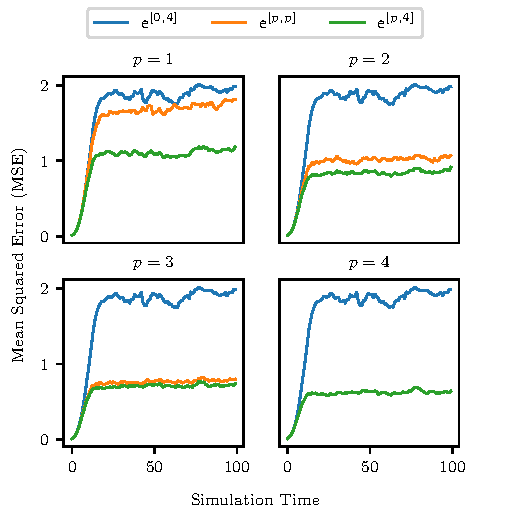
\includegraphics{figures/mse_privs.pdf}
  \caption{Average error of $1000$ simulation runs for different estimators when $\Sigma_z=2$ and $\Sigma_y=10$.}
  \label{fig:mse_privs}
\end{figure}
To demonstrate the effect of parameters $\Sigma_z$ and $\Sigma_y$ (and therefore $\mat{Z}$ and $\mat{Y}$), figure \ref{fig:mse_params} shows their effect on the average error of the same estimators. It can be seen that $\Sigma_z$ has a larger effect on the DKLB while $\Sigma_y$ has a larger effect on the SKUB. However, it can also be observed that both parameters affect both bounds to a degree, revealing some of the limitations of the proposed scheme.
\begin{figure}[htbp]
  \centering
  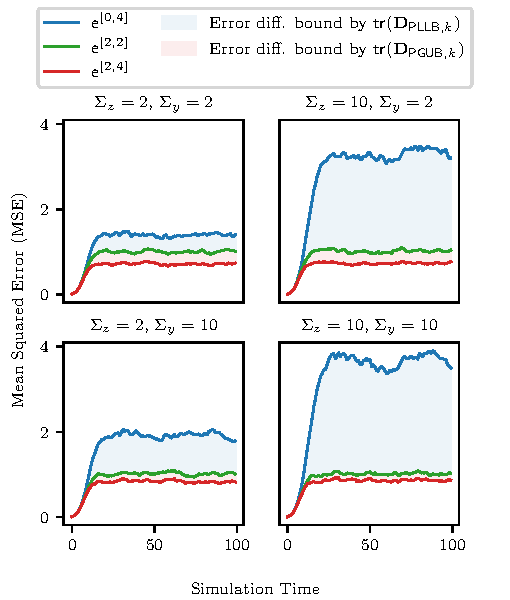
\includegraphics{figures/mse_params.pdf}
  \caption{Average error of $1000$ simulation runs of unprivileged and privilege-$2$ estimators for varying $\Sigma_z$ and $\Sigma_y$.}
  \label{fig:mse_params}
\end{figure}
Figure \ref{fig:trace_params} further captures this relation between the bounds and parameters $\Sigma_z$ and $\Sigma_y$. As the simulated system is asymptotically stable, steady state error covariances are reached. Traces of these covariances let us see the change in the steady state traces of the DKLB series(difference between blue and orange lines) and the SKUB series (difference between green and orange lines) when the parameters are changed. The larger effect of $\Sigma_z$ on the DKLB than $\Sigma_y$ can be clearly seen (steeper blue line when varying $\Sigma_z$), 

while the effects on the SKUB differ in that 

rate at which asymptotic 

% mention why unpriv can be better than pp


\begin{figure}[htbp]
  \centering
  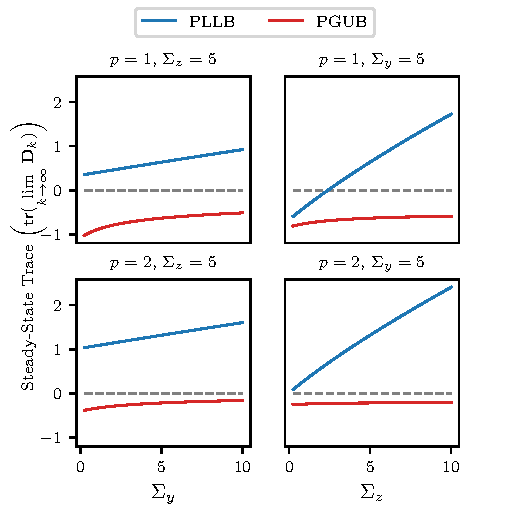
\includegraphics{figures/trace_params.pdf}
  \caption{Steady state trace of estiator error covariances for privileges $1$ and $2$ when $\Sigma_z$ and $\Sigma_y$ are varied.}
  \label{fig:trace_params}
\end{figure}

The relation between the correlated and uncorrelated components $\mat{Z}$ and $\mat{Y}$ mean that care must be taken when choosing the parameters to provide desired bounds between estimators

% 
%  .d8888b.   .d88888b.  888b    888  .d8888b.  
% d88P  Y88b d88P" "Y88b 8888b   888 d88P  Y88b 
% 888    888 888     888 88888b  888 888    888 
% 888        888     888 888Y88b 888 888        
% 888        888     888 888 Y88b888 888        
% 888    888 888     888 888  Y88888 888    888 
% Y88b  d88P Y88b. .d88P 888   Y8888 Y88b  d88P 
%  "Y8888P"   "Y88888P"  888    Y888  "Y8888P"  
%                                               
%                                               
%                                               
% 

\section{Conclusion}\label{sec:conc}
\begin{itemize}
  \item Concluding remarks.
  \item Future work includes exploring key subsets that do not need to be sequential, decentralised methods for multi-key correlated noise generation, and the effects and cryptographic guarantees of sensors falling out of synchronisation.
\end{itemize}

% conference papers do not normally have an appendix

% trigger a \newpage just before the given reference
% number - used to balance the columns on the last page
% adjust value as needed - may need to be readjusted if
% the document is modified later
%\IEEEtriggeratref{8}
% The "triggered" command can be changed if desired:
%\IEEEtriggercmd{\enlargethispage{-5in}}

% 
% 8888888b.  8888888888 8888888888 .d8888b.  
% 888   Y88b 888        888       d88P  Y88b 
% 888    888 888        888       Y88b.      
% 888   d88P 8888888    8888888    "Y888b.   
% 8888888P"  888        888           "Y88b. 
% 888 T88b   888        888             "888 
% 888  T88b  888        888       Y88b  d88P 
% 888   T88b 8888888888 888        "Y8888P"  
%                                            
%                                            
%                                            
% 

\bibliographystyle{IEEEtran}
\bibliography{bibliography/PrivilegedFusion}

% that's all folks
\end{document}


